% Drawing 154/06-20 -- folder 154, batch 06, archive page 103 (PDF page 104).
% Transcription: au-dessous, un tableau de dessins en couleur, en deux groupes à accolade marqués $\mathrm{I}$ et $\mathrm{II}$, chacun de deux lignes numérotées 1) et 2) : à gauche, deux paires de droites orange qui se croisent sur la droite vert clair $D$ ou au-dessus d'elle, orientée par $\omega$ (flèche vers la gauche), l'arc $a$ marqué au premier croisement et, en pointillé, l'arc $a'_0$ au second ; puis « donne », et à droite la position $D'$, orientée par $\omega'$, qui passe au-dessus du premier croisement (groupe $\mathrm{I}$) ou au-dessous (groupe $\mathrm{II}$), l'arc $b$ marqué en pointillé au premier croisement et l'arc $a'$ au second
% Kind: table of sweeps: D with omega gives D' with omega'. Method 2 (schematic redraw from the facsimile). Status: ok.
% Notes: Four rows. In each: on the left two orange crossings on D (or with D passing under them), the black arc a at the first, the dotted arc a'_0 at the second, the letter D, the arrow omega pointing left; the word « donne »; on the right D' making a bump over the first crossing (rows of I) or a dip under it (rows of II), the dotted arc b on the bump, the black arc a' at the second crossing, the letter D', the arrow omega' (to the right in the first three rows, to the left in the last). In row I.2 one stroke of the second crossing is gone over in black on the page, drawn like the others here; in row II.1 the line D is dark green. Crossings computed, every stroke through them; the brace groups I, II and the numbers 1), 2) at the left. Redrawn 2026-11-12 (issue 128): to check again.
% Coordinates: 1 unit = 1 mm = 1/100 of the crop width (bbox in page fractions: [0.21, 0.335, 0.63, 0.525]).
% Redrawn by Claude (claude-fable-5-2), issue #128, 2026-11-12; not checked by a human; not compiled (no TeX in the session).
% Rights: reproduces part of the work -- behind RENDER_TRANSCRIPTS, never published by itself.
\documentclass[tikz,border=3pt]{standalone}
\usepackage{amsmath,amssymb}
\usetikzlibrary{patterns,arrows.meta}
\tikzset{Or/.style={orange!90!black}, Lg/.style={green!60!black!70}, Dg/.style={green!45!black}, pencil/.style={black!45}, struck/.style={black!35}, mpt/.style={circle,draw,inner sep=1.3pt}, pt/.style={circle,fill,inner sep=0.9pt}, opt/.style={circle,draw,fill=white,inner sep=1.1pt}}
\begin{document}
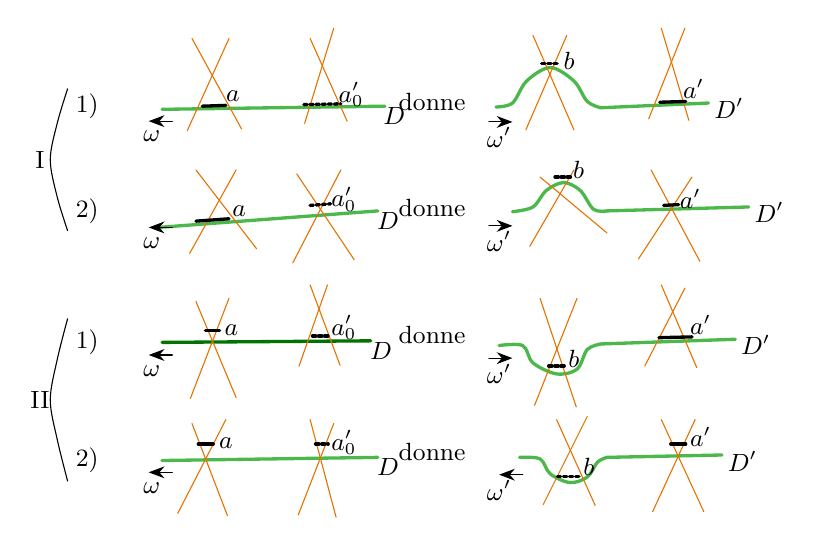
\begin{tikzpicture}[x=1mm,y=1mm,line cap=round,line join=round,font=\scriptsize]
\draw[Lg,very thick] (18.6,-13.7) -- (46.9,-13.3);
\draw[Or] (22.4,-4.7) -- (28.7,-16.2);
\draw[Or] (27.1,-4.7) -- (21.8,-16.4);
\draw[Or] (37.4,-4.7) -- (42.1,-15.2);
\draw[Or] (40.4,-3.4) -- (36.7,-15.5);
\draw[very thick] (23.7,-13.3) -- (26.7,-13.2);
\draw[densely dotted,very thick] (36.6,-13.1) -- (41.3,-13);
\node[inner sep=1pt] at (27.6,-12) {\small $a$};
\node[inner sep=1pt] at (42.6,-11.8) {\small $a'_0$};
\node[inner sep=1pt] at (48.1,-14.6) {\small $D$};
\draw[-{Stealth[length=2mm]}] (19.9,-15.2) -- (16.9,-15.2);
\node[inner sep=1pt] at (17.3,-17.1) {\small $\omega$};
\draw[Lg,very thick] plot[smooth, tension=0.55] coordinates {(61,-13.4) (63.1,-12.9) (64.9,-10.1) (67.9,-8.4) (70.9,-10.1) (72.6,-12.7) (74.3,-13.5)};
\draw[Lg,very thick] (74.3,-13.5) -- (88,-12.9);
\draw[Or] (65.7,-4.3) -- (70.9,-16.3);
\draw[Or] (70,-4.3) -- (64.8,-16.3);
\draw[Or] (82,-3.4) -- (85.5,-15.1);
\draw[Or] (85,-3.4) -- (80.4,-14.9);
\draw[densely dotted,very thick] (66.8,-7.9) -- (69.1,-7.9);
\draw[very thick] (81.8,-12.8) -- (85.1,-12.7);
\node[inner sep=1pt] at (70.3,-7.5) {\small $b$};
\node[inner sep=1pt] at (86.1,-11.1) {\small $a'$};
\node[inner sep=1pt] at (90.6,-13.6) {\small $D'$};
\draw[-{Stealth[length=2mm]}] (60.1,-15.3) -- (63.1,-15.3);
\node[inner sep=1pt] at (61.4,-17.3) {\small $\omega'$};
\draw[Lg,very thick] (18.1,-28.7) -- (46,-26.6);
\draw[Or] (22.9,-21.4) -- (30.6,-31.4);
\draw[Or] (28,-21.4) -- (22.1,-32);
\draw[Or] (35.7,-21.9) -- (43,-32.8);
\draw[Or] (41.3,-21.4) -- (35.2,-33.2);
\draw[very thick] (22.9,-27.9) -- (27.1,-27.6);
\draw[densely dotted,very thick] (37.4,-25.9) -- (40,-25.7);
\node[inner sep=1pt] at (28.4,-26.6) {\small $a$};
\node[inner sep=1pt] at (41.7,-25.1) {\small $a'_0$};
\node[inner sep=1pt] at (47.3,-27.9) {\small $D$};
\draw[-{Stealth[length=2mm]}] (19.9,-28.7) -- (16.9,-28.7);
\node[inner sep=1pt] at (17.3,-30.7) {\small $\omega$};
\draw[Lg,very thick] plot[smooth, tension=0.55] coordinates {(63.1,-26.7) (65.7,-26.1) (67.4,-24) (69.6,-23) (71.7,-24) (73.4,-26.4) (75.1,-26.6)};
\draw[Lg,very thick] (75.1,-26.6) -- (93.1,-26.1);
\draw[Or] (66.6,-22.3) -- (75.1,-29.4);
\draw[Or] (70.9,-21.4) -- (65.3,-31.1);
\draw[Or] (80.7,-21.4) -- (86.9,-33);
\draw[Or] (85.9,-22.3) -- (79.1,-32.7);
\draw[densely dotted,very thick] (68.5,-22.3) -- (70.5,-22.3);
\draw[very thick] (82.3,-25.9) -- (84.2,-25.8);
\node[inner sep=1pt] at (71.5,-21.4) {\small $b$};
\node[inner sep=1pt] at (85.7,-25.1) {\small $a'$};
\node[inner sep=1pt] at (95.7,-26.8) {\small $D'$};
\draw[-{Stealth[length=2mm]}] (60.1,-28.5) -- (63.1,-28.5);
\node[inner sep=1pt] at (61.4,-30.5) {\small $\omega'$};
\draw[Dg,very thick] (18.6,-43.3) -- (45.1,-43.1);
\draw[Or] (22.9,-38.1) -- (28,-50.3);
\draw[Or] (27.1,-37.7) -- (22.2,-50.4);
\draw[Or] (37.4,-36) -- (41.2,-46.2);
\draw[Or] (39.6,-36) -- (36,-46.3);
\draw[very thick] (24.1,-41.8) -- (25.9,-41.8);
\draw[densely dotted,very thick] (37.7,-42.5) -- (40,-42.5);
\node[inner sep=1pt] at (27.4,-41.7) {\small $a$};
\node[inner sep=1pt] at (41.7,-41.4) {\small $a'_0$};
\node[inner sep=1pt] at (46.4,-44.4) {\small $D$};
\draw[-{Stealth[length=2mm]}] (19.9,-44.9) -- (16.9,-44.9);
\node[inner sep=1pt] at (17.3,-46.9) {\small $\omega$};
\draw[Lg,very thick] plot[smooth, tension=0.55] coordinates {(61.4,-43.7) (64.4,-43.7) (65.7,-45.9) (68.7,-47.3) (71.3,-46.7) (72.6,-44.2) (74.3,-43.5)};
\draw[Lg,very thick] (74.3,-43.5) -- (91.4,-42.9);
\draw[Or] (66.6,-37.7) -- (71.2,-51.5);
\draw[Or] (71.3,-37.7) -- (65.9,-51.3);
\draw[Or] (82,-36) -- (86.5,-46.5);
\draw[Or] (85,-36.4) -- (79.9,-46.3);
\draw[densely dotted,very thick] (67.7,-46.3) -- (70,-46.3);
\draw[very thick] (81.7,-42.7) -- (85.9,-42.6);
\node[inner sep=1pt] at (70.9,-45.4) {\small $b$};
\node[inner sep=1pt] at (87,-41.1) {\small $a'$};
\node[inner sep=1pt] at (94,-43.6) {\small $D'$};
\draw[-{Stealth[length=2mm]}] (60.1,-45.3) -- (63.1,-45.3);
\node[inner sep=1pt] at (61.4,-47.3) {\small $\omega'$};
\draw[Lg,very thick] (18.6,-58.3) -- (46,-57.9);
\draw[Or] (22.4,-53.6) -- (26.9,-65.3);
\draw[Or] (26.7,-53.1) -- (20.6,-65);
\draw[Or] (37.4,-53.1) -- (40.7,-65.5);
\draw[Or] (40.4,-53.6) -- (35.9,-65.2);
\draw[very thick] (23.2,-56.2) -- (25.1,-56.2);
\draw[densely dotted,very thick] (38.1,-56.2) -- (39.7,-56.2);
\node[inner sep=1pt] at (26.7,-56.1) {\small $a$};
\node[inner sep=1pt] at (41.7,-56) {\small $a'_0$};
\node[inner sep=1pt] at (47.3,-59.1) {\small $D$};
\draw[-{Stealth[length=2mm]}] (19.9,-59.8) -- (16.9,-59.8);
\node[inner sep=1pt] at (17.3,-61.8) {\small $\omega$};
\draw[Lg,very thick] plot[smooth, tension=0.55] coordinates {(64,-57.9) (66.6,-58.1) (67.9,-60) (70.4,-61.1) (72.6,-60.4) (73.9,-58.5) (75.1,-57.9)};
\draw[Lg,very thick] (75.1,-57.9) -- (89.7,-57.6);
\draw[Or] (68.7,-53.1) -- (73.6,-64);
\draw[Or] (72.6,-52.7) -- (67,-63.9);
\draw[Or] (82,-53.1) -- (87.4,-64.8);
\draw[Or] (86.3,-53.1) -- (80.9,-64.8);
\draw[densely dotted,very thick] (68.8,-60.3) -- (71.7,-60.3);
\draw[very thick] (83.2,-56.2) -- (85.1,-56.2);
\node[inner sep=1pt] at (72.8,-59.1) {\small $b$};
\node[inner sep=1pt] at (87,-55.3) {\small $a'$};
\node[inner sep=1pt] at (92.3,-58.4) {\small $D'$};
\draw[-{Stealth[length=2mm]}] (64.4,-60.1) -- (61.4,-60.1);
\node[inner sep=1pt] at (61.4,-62.1) {\small $\omega'$};
\node[inner sep=1pt] at (52.9,-12.7) {\small donne};
\node[inner sep=1pt] at (52.9,-26.2) {\small donne};
\node[inner sep=1pt] at (52.9,-42.3) {\small donne};
\node[inner sep=1pt] at (52.9,-57.2) {\small donne};
\node[inner sep=1pt] at (3.1,-20.1) {\small $\mathrm{I}$};
\node[inner sep=1pt] at (3.1,-50.6) {\small $\mathrm{II}$};
\node[inner sep=1pt] at (9.1,-13.3) {\small 1)};
\node[inner sep=1pt] at (9.1,-26.6) {\small 2)};
\node[inner sep=1pt] at (9.1,-43.3) {\small 1)};
\node[inner sep=1pt] at (9.1,-58.3) {\small 2)};
\draw plot[smooth, tension=0.55] coordinates {(6.6,-11.1) (5.3,-15.4) (4.4,-20.1) (5.3,-24.9) (6.6,-29.1)};
\draw plot[smooth, tension=0.55] coordinates {(6.6,-40.3) (5.3,-45.4) (4.4,-50.6) (5.3,-55.7) (6.6,-60.9)};
\end{tikzpicture}
\end{document}
